\documentclass[uplatex]{jsarticle}
%\documentclass[a4j]{ujarticle}
\usepackage{resume}  % resume用スタイル
\usepackage{udline}  % 下線用
\usepackage{comment} % 複数行コメント
\usepackage{multirow} % セル統合
\usepackage{makecell} % セル内で改行するため
% \usepackage{siunitx}  % 数式フォントを本文フォントにそろえるため

\pagestyle{plain}

\begin{document}
\twocolumn[
    \beginheader{令和7年度 コンピュータサイエンス学部 中間発表}{2025}{8}{7}{井上 研究室}
    \title{握り操作によるVR武器切替コントローラの提案}
    \author{C0B22045 川地 道人 (Michito Kawachi)}
    \endheader
]
\vspace{3mm}

%%ページ番号
\setcounter{page}{15}

\section{はじめに}

VRゲームをプレイする際,プレイヤーは左右にコントローラを握る.
自分のキャラクターはプレイヤーの現実での動作に同期して動く.
現実とVRとの感覚に差がないと,高い没入感を得ることができる.

コントローラも,現実との差を埋めるために有効なデバイスだ.
現実でVR内の武器に似せた物を持つことで,特に触覚に働きかけ,高い没入感が得られる.
しかしVRで使われる武器の種類が多いため,それぞれに一対一対応する専用コントローラを用意することは一般的でない.
また,専用コントローラを用意できたとしても,現在把持しているコントローラを放し,別のコントローラを探して持つことは,ゲーム体験を中断させる.

そこで1つのコントローラで多くの武器に対応できるデバイスが研究されてきた.


\section{関連研究}


市川らは,武器選択の簡略化と現実とVRでの武器の把持状態を一致させることを目的として,ConcateRoller(\figref{fig:ConcateRoller_concate})を提案した\cite{市川2025ConcateRoller}.
ConcateRollerは,左右で把持するコントローラを合体・分離する機構を有するコントローラである.
合体状態で両手持ちする武器の把持姿勢を,分離状態で片手持ちする武器の把持姿勢を再現した.
% ConcateRollerを既存の汎用コントローラに取り付け,縦に合体させることで,現実とVRでのアイテムの把持形態を一致させる.
% 合体状態では両手で操作するアイテムだけを,分離状態では片手で操作するアイテムだけが選択肢に取ることができる.
% プレイヤー体験に関する実験の結果,ConcateRollerを使った武器切り替えにおいて,体験に与える影響の有無は有意に示されなかった.
% これはConcateRollerを合体させる動きがスムーズにできないからだと考察している.
% VRと現実の把持形態の一致を目的としているが,アイテムの持ち手の太さを提示することは扱っていない.
しかし,武器は持ち方以外にも様々なプロパティがある.
武器の大きさは全体を触って確認しなければならないが,太さは持っているだけで認識することができる.
ConcateRollerでは大きな武器も小さな武器も同じ太さであるため,それでは没入感が上がらないと考えた.
% 太さの差を提示できていない.

% 現実で両手持ちする物体は,頭パーツが重いため,両手持ちする理由があり,持ち手が太く丈夫に作られていることが多い.


\begin{figure}[htbp]
    \centering
    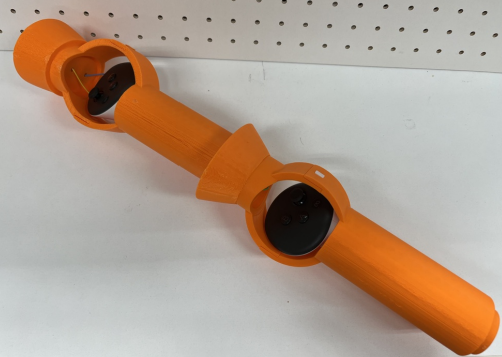
\includegraphics[width=0.9\linewidth]{fig/ConcateRoller合体.png}
    \caption{合体状態のConcateRoller}
    \label{fig:ConcateRoller_concate}
\end{figure}

Gonzalez らはVR内の物体の形状を触覚提示できるデバイスとして,X-Rings(\figref{fig:X-Rings})を提案した\cite{gonzalez2021x-rings}.
X-Ringsは手全体で握れるデバイスで,5.5cmから7.7cmに拡張可能なリングが4つ積み重ねられている.
それぞれが自由に変形するため,コップの形状やくびれのあるボトルの形状など,1つのデバイスで幅広いオブジェクトの触覚を提示することができる.
しかし,システムにより形状を変化させるだけで,ユーザが自由に太さを変化させることはできない.
本研究ではユーザからの入力が主体となるため,X-Ringsでは太さによる武器切り替えができない.

\begin{figure}[htbp]
    \centering
    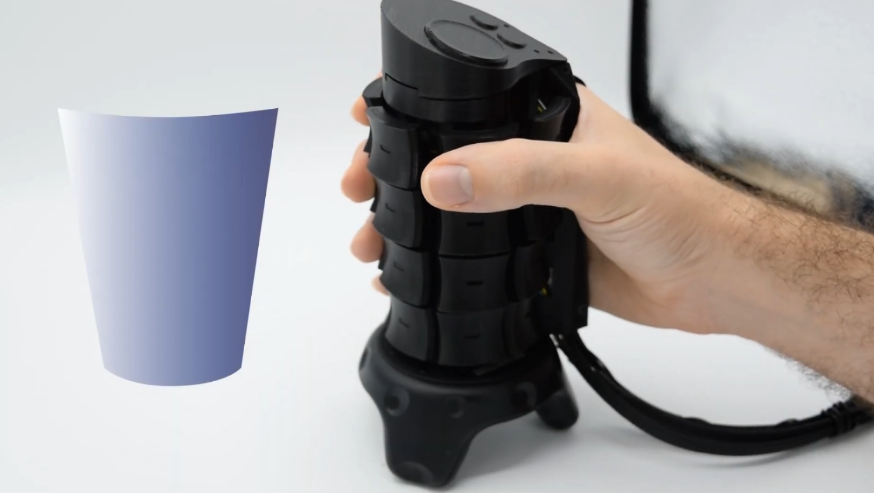
\includegraphics[width=0.9\linewidth]{fig/X-Rings.png}
    \caption{コップの形状を再現するX-Rings}
    \label{fig:X-Rings}
\end{figure}


\section{握り操作により持つ武器を切り替えるコントローラ}

\subsection{システム概要}

システム構成を\figref{fig:system}に示す.
コントローラの現在の太さをPCが推定して,対応した武器に切り替わるようにVRに信号を送る.
図のようにコントローラを1番太い状態にすると,VR内では自動でハンマーのような一番太い武器に切り替わる.
同様にコントローラを2番目に太い武器では剣,最も細い状態にすると杖というように切り替えることができる.

コントローラとPCは無線接続を検討している.
ユーザが自由に動かせることで没入感に影響すると考えたからだ.

\begin{figure}
    \centering
    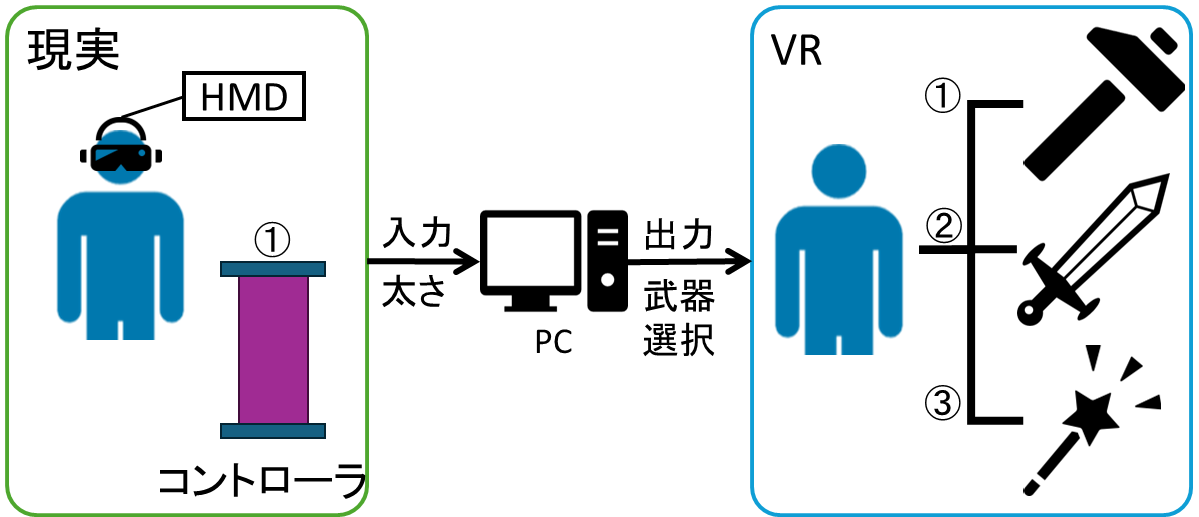
\includegraphics[width=0.9\linewidth]{fig/構成図.png}
    \caption{システム概要}
    \label{fig:system}
\end{figure}


\subsection{太さ変形機構}

\figref{fig:Zentai}にコントローラの全体を示す.
このコントローラは,上部と下部のゼンマイばねと中心軸,ユーザが握る4本の紫色の円柱で構成される.
図に示した2つの状態とさらに細い1段階を加え,3段階の太さで操作する.
ユーザが4本の紫の円柱を握り,中心にスライドさせることで,太さを変化させられる.

\begin{figure}[htbp]
    \centering
    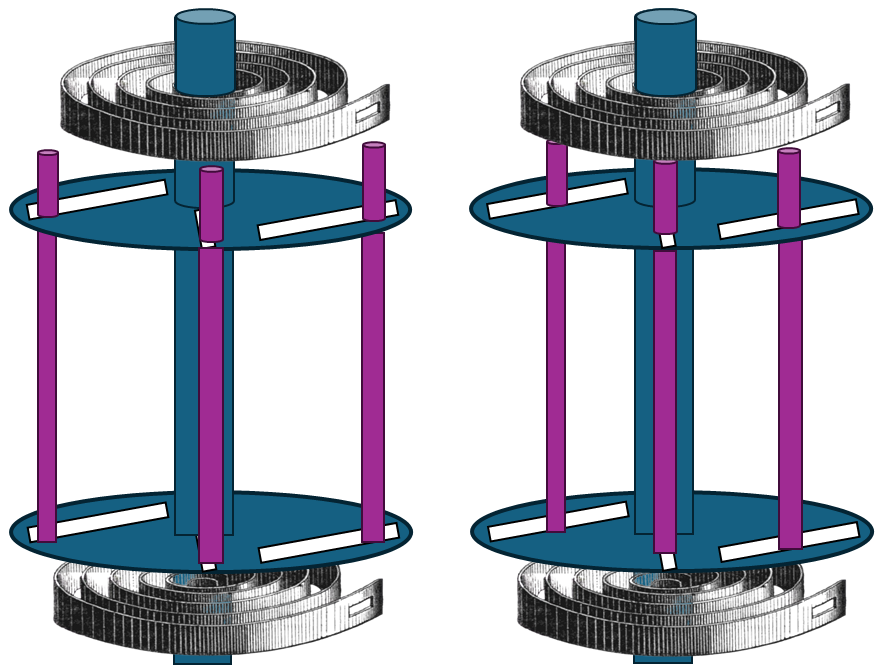
\includegraphics[width=0.7\linewidth]{fig/横からみた図.png}
    \caption{コントローラを横からみた図(左図は1番太い状態.右図は2番目に太い状態.)}
    \label{fig:Zentai}
\end{figure}

\figref{fig:SlashGear}にユーザが握る円柱を支える円盤構造を示す.
中心の円はコントローラを貫く中心軸を,4つの紫の円はユーザが握る部分(以下4本柱)を表す.
白い部分は円盤に穴が開いていることを表す.
4本柱は円盤の穴に沿って,それぞれ中心軸に対して放射状に移動する.

\begin{figure}[htbp]
    \centering
    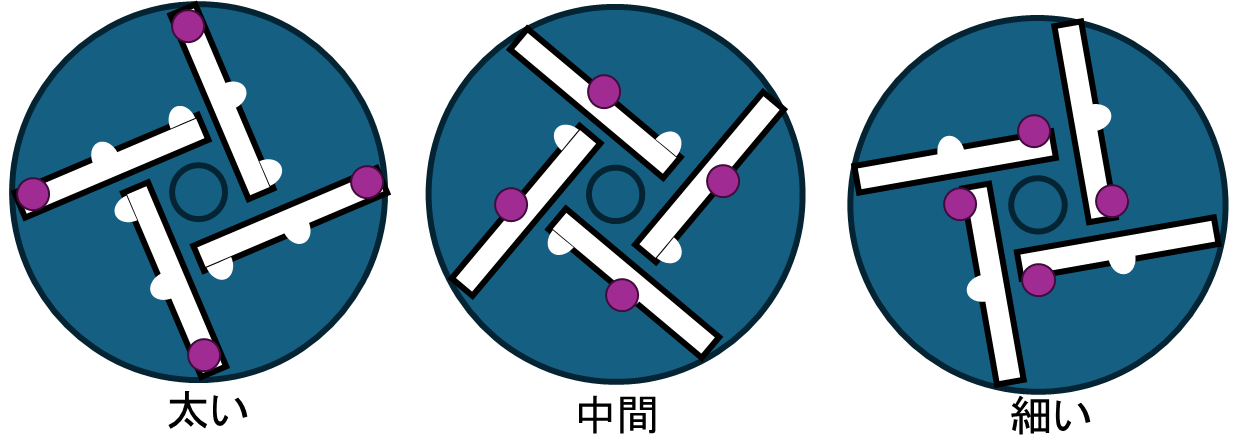
\includegraphics[width=0.9\linewidth]{fig/太さ3段階.png}
    \caption{太さを変更する機構}
    \label{fig:SlashGear}
\end{figure}

1番太い状態から2番目に太い状態になるときの変化を例に,4本柱の動きを説明する.
ユーザが4本柱を握って細くしようとすると,レーンの切り欠きがない面に押し付けられるように滑る.
円盤は固定されていないため,反時計回り方向に回転する.
このとき,中心軸に固定されたゼンマイばねが圧縮され,一番太い状態への復元力が蓄積される.
中心軸から遠い切り欠きを少し通り過ぎてから手を緩めると,ゼンマイばねの復元力によって,円盤が時計回りに回転する.
4本柱が中心軸から離れるようにレーンに押され,中心から遠い方の切り欠きに引っ掛かりロックされる(\figref{fig:SlashGear}の中央).

コントローラを太くするときは,ロックからレーンに戻し,握る力を弱める.
するとばねの復元力で円盤が時計回りに回転し,レーンに沿って4本柱が外側へ動く.
% 上下のゼンマイばねによって4本柱に常に外側に戻る方向の力が働くため,この機構は太さ変更のために電子部品を必要としない.

機構の検討事項を示す.
1つ目は現在の太さの検知方法だ.
ロータリーエンコーダを使う方法と,切り欠きと,4本柱のロック機構と同じ高さに銅箔テープを巻き,接触しているかで検知する方法の2つを検討している.
2つ目はロック機構の解除方法だ.
現状4本柱を同じ太さにとどめる機構は提案できたが,ロックを解除する方法については考慮が必要だ.
切り欠きから内側に力を与える方法か,切り欠きを埋めるパーツで押し出す方法の2つを検討している.


\section{評価方法}

ユーザにHMDとコントローラを装着させ,指定された武器で目標を切ってもらう実験を実施する.
武器の選択方法を,提案手法と既存のVRコントローラを使う方法の2種類についてそれぞれ行う.
被験者は実験後,没入感や使いやすさに関するアンケートに回答する.

定量評価として,武器の切り替えにかかった時間,武器を間違えて攻撃した回数,タスクにかかった時間を計測する.
定性評価として,没入感や使いやすさ,掌から感じた太さと視覚から感じた太さの乖離について,5段階のリッカートスケールで評価する.

\section{まとめ}

本研究では,持ち手の太さで武器を切り替えられる操作手法を提案した.
視覚と触覚の差を埋めることで,没入感の高いコントローラを開発できると考えている.



\bibliographystyle{junsrt}
\bibliography{ref}

\end{document}